\newpage
\section{Register Allocation}
通过染色算法对冲突图求解.
\subsection{Coloring by Simplification}
寄存器分配与图染色都是 NP-complete 问题. 这里使用一种线性近似算法, 分为构建, 简化, 溢出, 选择四个阶段. 

\begin{enumerate}
    \item 构建: 构建冲突图.
    \item 简化: 启发式图染色. 将图中度数 $<K$ (寄存器个数) 的节点删除, 并压入一个栈中. 直到剩下节点度数都 $\ge K$, 无法继续简化. 
    \item 溢出: 称目前剩下为高度数(significant degree, 度$\ge K$)点. 选择与剩下其他节点无冲突的, 代表临时变量的点作为溢出, 将其删除并标记为潜在溢出(potential spill)压入栈中. 然后继续简化. 
    \item 选择: 从空图开始, 将点从栈中弹出, 加入到图中并染色.  每次加入节点, 其必须被染色. 
    \subitem 若为潜在溢出的点, 其可能无法被染色, 则将其标记为实际溢出(actual spill), 然后不管其继续弹出节点. 
    \subitem 但潜在溢出的点也可能被成功染色(其周围有节点颜色相同), 此时称为乐观染色(optimistic coloring).
    \item 重开: 对实际溢出的节点, 重写程序通过读写内存对其进行操作. 但就算如此, 读写也需要额外几个临时寄存器, 此时对于重写的程序, 重新构建冲突图, 跑染色算法. 多次迭代直到简化阶段不会溢出, 一般而言, 一两次迭代即可. 
\end{enumerate}

假设 $a$ 发生了实际溢出, 则 $a$ 必须通过读写内存对其进行操作. 对其 def 与 use 的修改如下:
\begin{enumerate}
    \item 对于 $a$ 的每个 use, 新建 $a_i$, 从 $M[a_{loc}]$ 读取 $a$. 
    \subitem $c\leftarrow a \Rightarrow a_1\leftarrow M[a_{loc}], c\leftarrow a_1$
    \item 对于 $a$ 的每个 def, 新建 $a_i$, 通过其写入 $M[a_{loc}]$.
    \subitem $a\leftarrow c \Rightarrow a_2\leftarrow c, M[a_{loc}]\leftarrow a_2$
\end{enumerate}

\begin{example}
    假设有四个寄存器. 

    \begin{figure}[!htb]
        \centering
        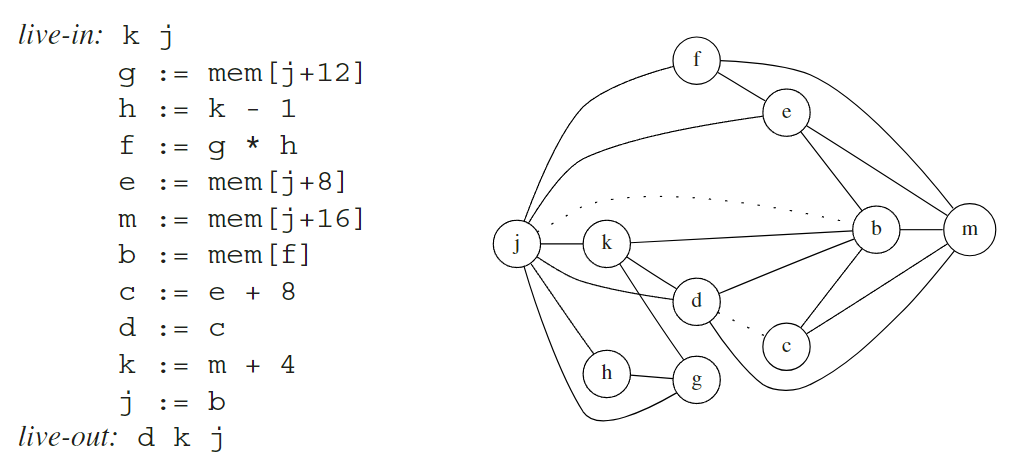
\includegraphics[width=0.42\textwidth]{pic/CP11/Interference graph for a program}
        \caption{Interference graph for a program}
        \label{fig:Interference-graph}
    \end{figure}
    
    \textbf{Figure} \ref{fig:Interference-graph} 简化就可以删除全部节点了. 然后依次弹出并染色. 

    \begin{figure}[!htb]
        \centering
        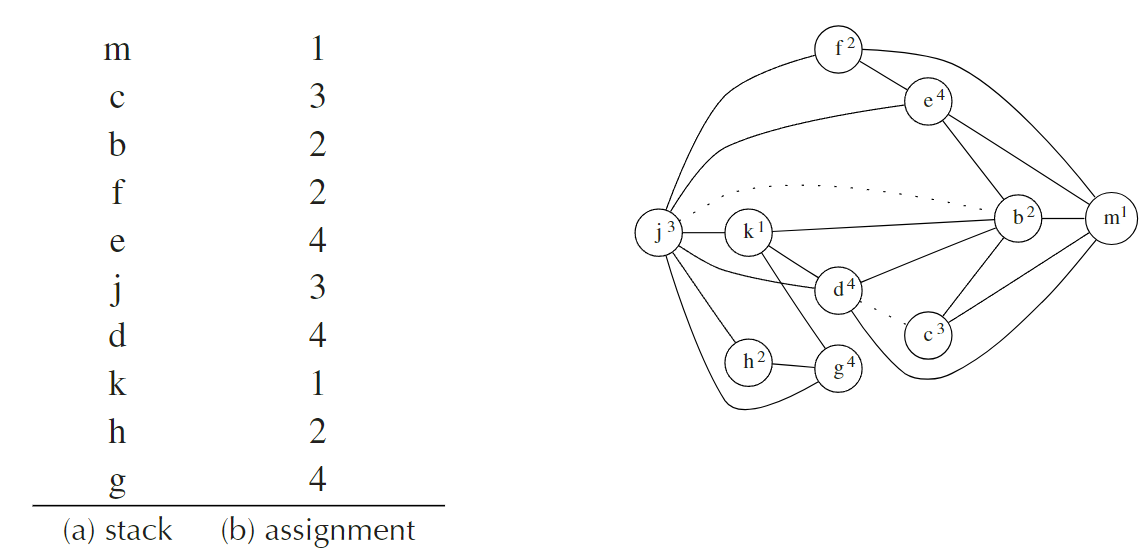
\includegraphics[width=0.42\textwidth]{pic/CP11/Simplification stack, and a possible coloring}
        \caption{Simplification stack, and a possible coloring}
    \end{figure}
    
    
\end{example}

\subsection{Coalescing}
删除冗余的 MOVE 指令. 若 MOVE 的 src 与 dst 之间不冲突, 则将其合并为新节点, 与新节点冲突的点是二者的并集. 理论上, 任意一对不冲突的点都可以被合并. 但合并可能导致原本可被染色图不能被染色. 

所以引出安全的合并策略:
\begin{enumerate}
    \item Briggs: 如果 $a,b$ 合并后的节点 $ab$ 的高度数邻居个数 $<K$,则 $a, b$ 可以合并.
    \item George: 对于 $a$ 的每个邻居 $t$, 若 $t$ 与 $b$ 冲突, 或者 $t$ 是低度数点(度$<K$), 则 $a,b$ 可以合并. 
\end{enumerate}

这 两 种 策 略 都 是 保 守 的(conservative), 因 为其合并不会改变图的着色性. 策略执行后可能仍有多余的 MOVE 指令, 但这至少比溢出好.


\begin{figure}[!htb]
    \centering
    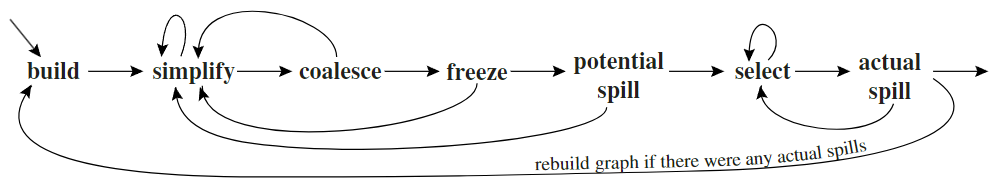
\includegraphics[width=0.42\textwidth]{pic/CP11/Graph coloring with coalescing}
    \caption{Graph coloring with coalescing}
\end{figure}

带合并的图染色算法:
\begin{enumerate}
    \item 构建: 构建冲突图, 将节点分类为 move-related 与 non-move-related. move-related 节点指此点是 MOVE 的 src 或 dst. 
    \item 简化: 删除低度数($<K$) 的 non-move-related 节点, 并压入栈中. 直到无法简化. 
    \item 合并: 运行保守的合并策略, 每次合并两个节点(删除相关 MOVE 指令), 若结果是 non-move-related, 则继续简化. 重复简化合并直到剩下的都是高度数或 move-related 节点. 
    \item 冻结: 寻找一个度数较低的 move-related 节点, 放弃对其相关 MOVE 指令的合并, 将此 MOVE 指令相关的点标记为 non-move-related. 然后继续简化合并.
    \item 溢出: 若没有低度数节点, 选择高度数节点作为潜在溢出并删除压入栈中. 
    \item 选择:将点从栈中弹出, 加入到图中并染色. 
\end{enumerate}

\begin{example}
    仍是四个寄存器, 以 \textbf{Figure} \ref{fig:Interference-graph} 为例. 

    只有 $b,c,d,j$ 四个点是 move-related 的. 简化 $g,h,k$. 然后合并 $cd, bj$. 最后完成所有的简化. 不需要溢出. 

    \begin{figure}[!htb]
        \centering
        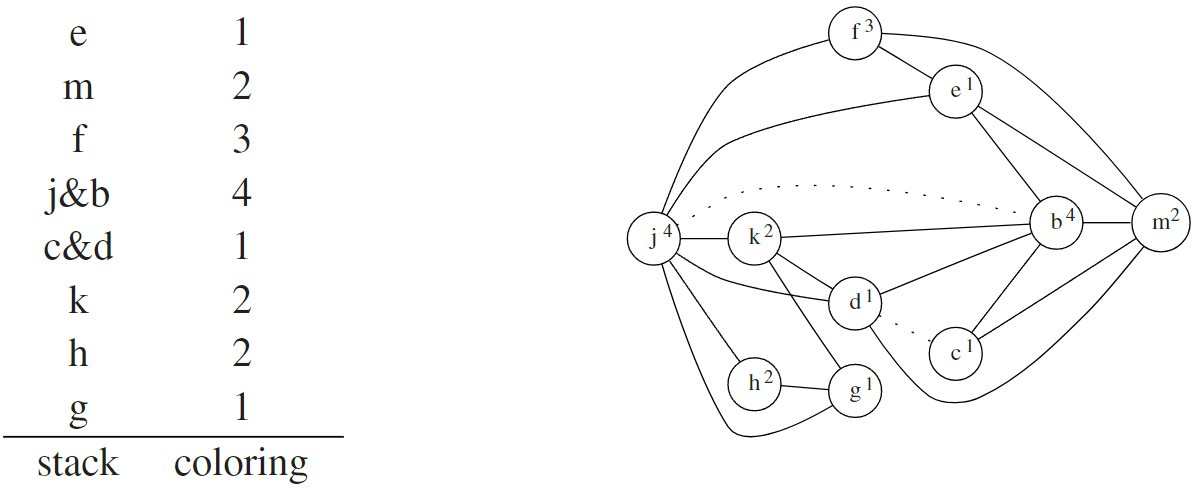
\includegraphics[width=0.42\textwidth]{pic/CP11/A coloring, with coalescing}
        \caption{A coloring, with coalescing}
    \end{figure}
    
\end{example} 

若冲突图中两个节点既有虚线又有实现, 则称之为受约束的(constrained). 对此不将其考虑为 move-related. 

\subsection{Precolored Nodes}
有一些临时变量是预着色的, 代表的是机器寄存器, 参数寄存器, 帧指针, 返回值寄存器等. 预着色的点必须相互冲突, 一般来说, 一个颜色只会对一个节点预着色. 

选择与合并操作可以给一个普通点被预着色的颜色, 只要没有冲突. 特别的, 当一个预着色节点与普通节点使用 George 合并时, 需要将普通节点作为 $a$, 检查普通节点的邻居是否满足合并条件. 

预着色节点特性:
\begin{enumerate}
    \item 无法简化
    \item 无法溢出(认为此点的度无限大)
    \item 可以参与合并.
\end{enumerate}

染色算法通过简化合并溢出来工作, 直到只剩下预着色节点, 然后才能开始向冲突图中加入其他节点. 预着色节点不能溢出所以前端必须使他们的活跃范围保持较小, 可以通过 MOVE 指令来实现. 

对于节点 $a$, 其溢出优先级计算公式: 
\begin{align*}
    Priority = \frac{Out_{use+def}+10\times In_{use+def}}{D}
\end{align*}
其中,
\begin{itemize}
    \item $Out_{use+def}$ 为 $a$ 在循环外的 use 与 def 总数.
    \item $In_{use+def}$ 为 $a$ 在循环内的 use 与 def 总数.
    \item $D$ 为 $a$ 的度, 只包含实线. 
\end{itemize}

优先级值越小, 说明优先级越高. 表示优先溢出不被经常使用的高度数节点. 

% \subsection{Graph Coloring Implementation} 这章讲如何具体实现算法, 考试不太可能考, 跳了.

% \subsection{Register Allocation for Trees} 也是讲代码, 跳了